\hypertarget{rainbow-room}{%
\section{Rainbow Room}\label{rainbow-room}}

\begin{figure}[!ht]
  \begin{adjustwidth}{-\oddsidemargin-1in}{-\rightmargin}
    \centering
    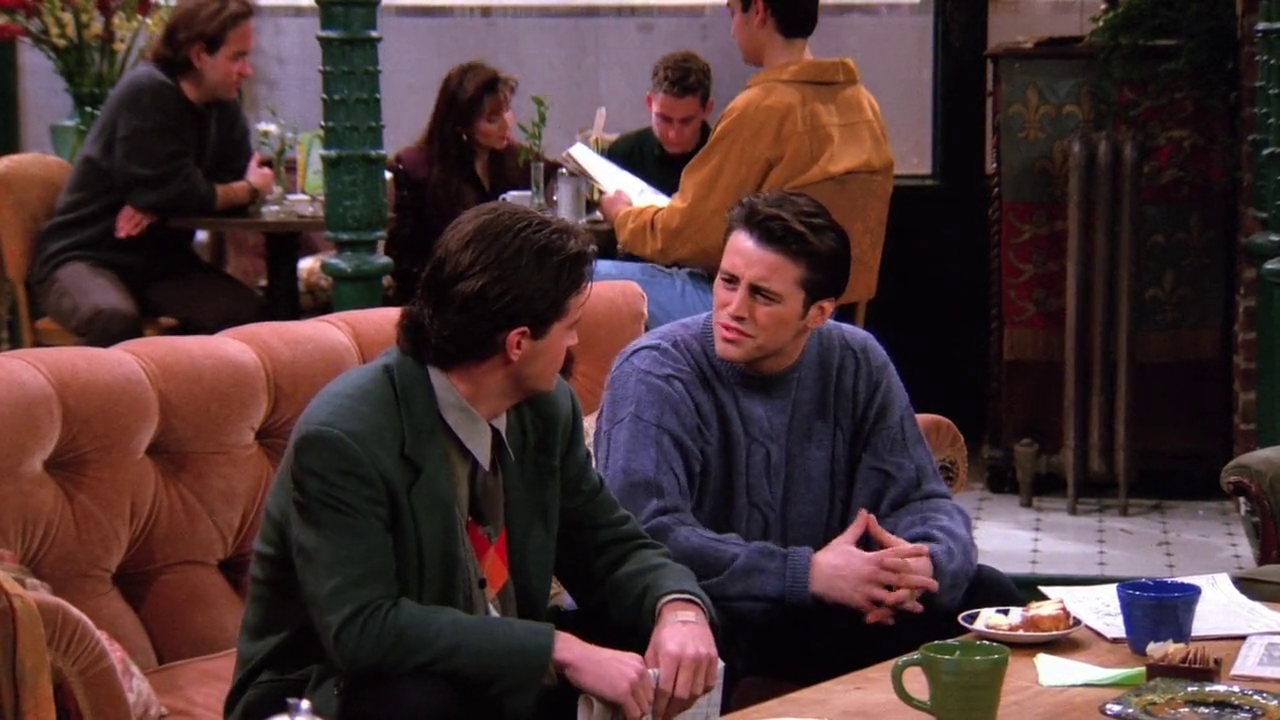
\includegraphics[trim={0 4cm 0 7cm,}, clip, width=\paperwidth]{./S01/img/17/rainbow-room.png}
    % \caption{Rainbow Room\label{fig:rainbow-room}}
  \end{adjustwidth}
\end{figure}

\begin{tcolorbox}[enhanced,center upper,
    drop fuzzy shadow southeast, boxrule=0.3pt,
    lower separated=false,
    colframe=black!30!dialogoBorder,colback=white]
\begin{minipage}[c]{0.16\linewidth}
  \raisebox{\dimexpr-\height+\ht\strutbox\relax}{
    \centering 
\includegraphics[width=1.4cm]{./assets/img/joey.png}
  }
   & \centering \scriptsize{Joey}
\end{minipage}
\hfill
\begin{minipage}[c]{0.8\linewidth}
  \textbf{- Have either of you ever been to the Rainbow Room? Is it expensive?}\\
  - Algum de vocês já foi ao Rainbow Room? É caro?
\end{minipage}

\medskip
\begin{minipage}[c]{0.16\linewidth}
  \raisebox{\dimexpr-\height+\ht\strutbox\relax}{
    \centering 
\includegraphics[width=1.4cm]{./assets/img/chandler.png}
  }
   & \centering \scriptsize{Chandler}
\end{minipage}
\hfill
\begin{minipage}[c]{0.8\linewidth}
  \textbf{- Only if you order stuff.}\\
  - Só se você pedir alguma coisa.
\end{minipage}
\end{tcolorbox}

Querendo levar Ursula a um local bacana em seu encontro Joey menciona o
\emph{Rainbow Room} (1934), salão para eventos situado no prédio
\emph{Rockefeller Plaza}, no centro de \emph{Manhattan} em Nova Iorque.
É um local realmente caro devido a sua localização, ambientação e
serviço de alimentação.

\begin{figure}
  \centering
  \begin{tikzpicture}
    \node [inner sep=0pt] at (0,0) {
      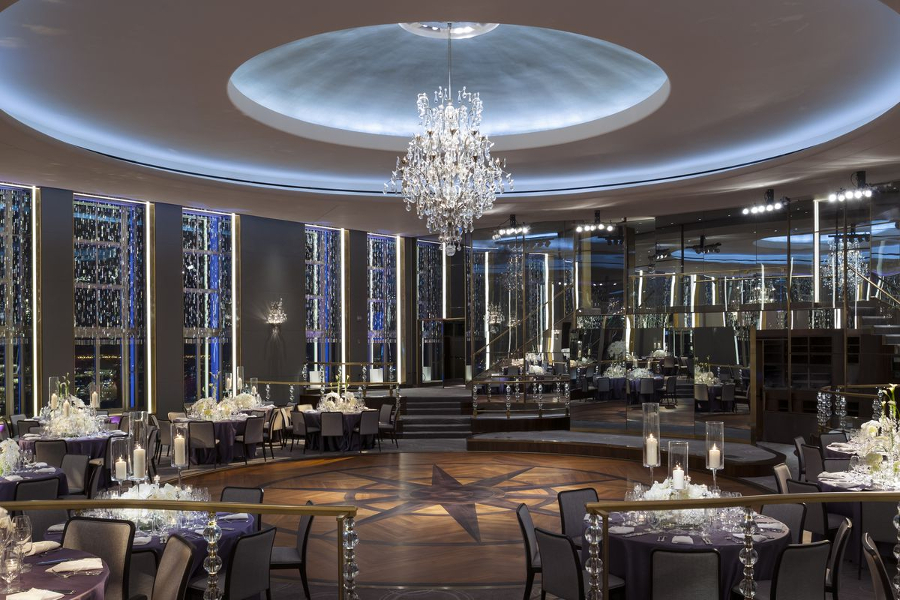
\includegraphics[width=0.8\textwidth,keepaspectratio]{./S01/img/17/rainbow-room-espaco.jpg}
    };
    \draw [white, rounded corners=\ClipSep, line width=\ClipSep]
    (current bounding box.north west) --
    (current bounding box.north east) --
    (current bounding box.south east) --
    (current bounding box.south west) -- cycle
    ;
    \end{tikzpicture}
    \caption{Rainbow Room - Espaço\label{fig:rainbow-room-espa-o}}
\end{figure}

\hypertarget{referuxeancias}{%
\subsection{Referências}\label{referuxeancias}}

\begin{itemize}
\tightlist
\item
  \sloppy Site oficial (Inglês). \url{https://rainbowroom.com/our-history/}
\end{itemize}

\hypertarget{colonial-williamsburg}{%
\section{Colonial Williamsburg}\label{colonial-williamsburg}}

\begin{figure}[!ht]
  \begin{adjustwidth}{-\oddsidemargin-1in}{-\rightmargin}
    \centering
    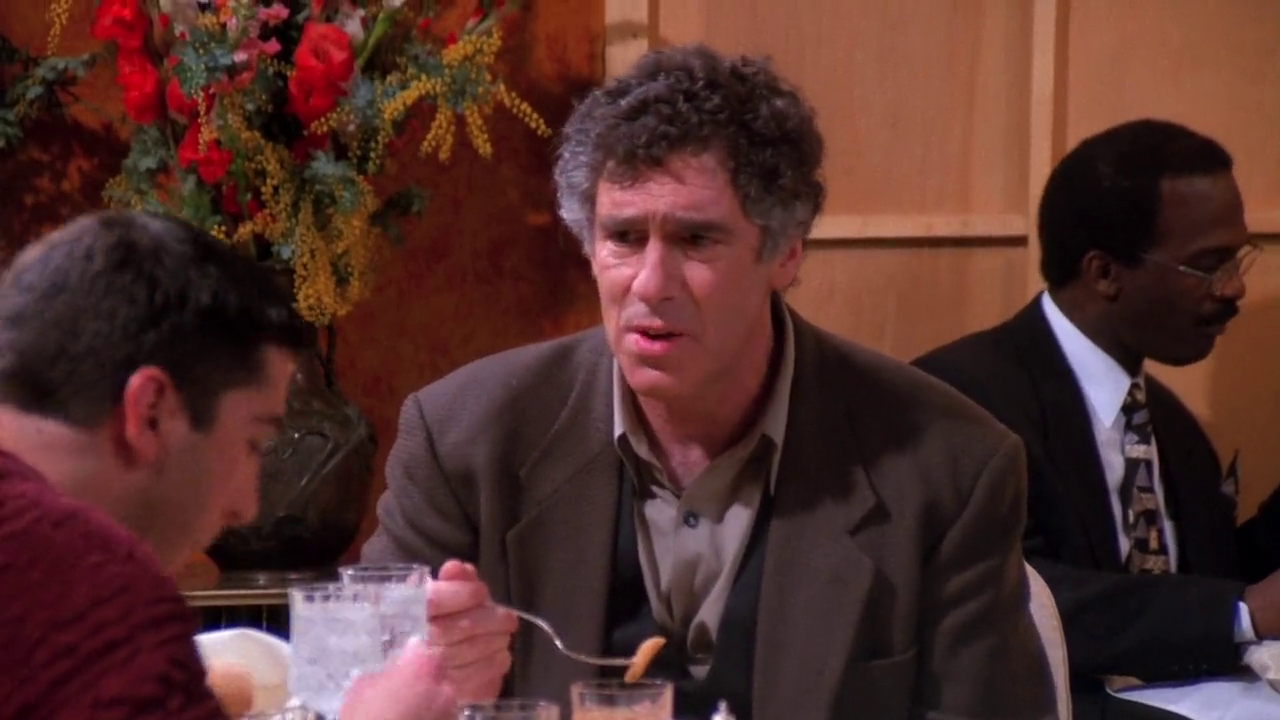
\includegraphics[trim={0 6cm 0 2cm,}, clip, width=\paperwidth]{./S01/img/17/colonial-williamsburg.png}
    % \caption{Colonial Williamsburg\label{fig:colonial-williamsburg}}
  \end{adjustwidth}
\end{figure}

\begin{tcolorbox}[enhanced,center upper,
    drop fuzzy shadow southeast, boxrule=0.3pt,
    lower separated=false,
    colframe=black!30!dialogoBorder,colback=white]
\begin{minipage}[c]{0.16\linewidth}
  \raisebox{\dimexpr-\height+\ht\strutbox\relax}{
    \centering 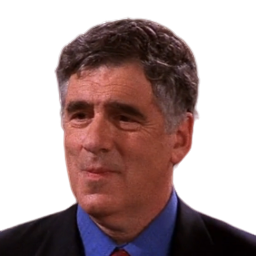
\includegraphics[width=1.4cm]{./assets/img/jack.png}
  }
   & \centering \scriptsize{Jack}
\end{minipage}
\hfill
\begin{minipage}[c]{0.8\linewidth}
  \textbf{- You always wanted to go to Colonial Williamsburg. How about we do that?}\\
  - Você sempre quis ir a Colonial Williamsburg. Que tal?
\end{minipage}
\end{tcolorbox}

Conversando com Ross sobre paternidade Jack o convida a ir para
\emph{Colonial Williamsburg} (1926), é o maior museu a céu aberto dos
EUA. Oferece uma autêntica experiência de como era o local no século
XVIII. O \emph{Reverendo Dr.~William Goodwin} com o apoio financeiro de
\emph{John D. Rockefeller Jr.} foram os responsáveis por restaurar
\emph{Williamsburg}, que tem, hoje, pelo menos 88 edificações originais.

\begin{figure}
  \centering
  \begin{tikzpicture}
    \node [inner sep=0pt] at (0,0) {
      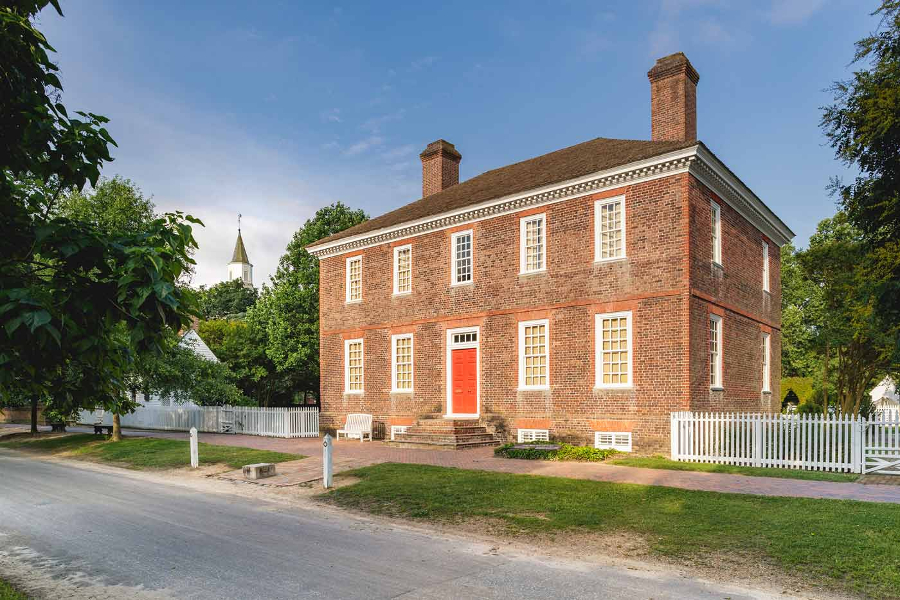
\includegraphics[width=0.8\textwidth,keepaspectratio]{./S01/img/17/colonial-williamsburg-wythe-house.jpg}
    };
    \draw [white, rounded corners=\ClipSep, line width=\ClipSep]
    (current bounding box.north west) --
    (current bounding box.north east) --
    (current bounding box.south east) --
    (current bounding box.south west) -- cycle
    ;
    \end{tikzpicture}
    \caption{Colonial Williamsburg - Wythe House\label{fig:colonial-williamsburg-wythe-house}}
\end{figure}

\hypertarget{referuxeancias-1}{%
\subsection{Referências}\label{referuxeancias-1}}

\begin{itemize}
\tightlist
\item
  \sloppy Site oficial (Inglês). \url{https://www.colonialwilliamsburg.org/learn/about-colonial-williamsburg/}
\end{itemize}

\hypertarget{love-connection}{%
\section{Love Connection}\label{love-connection}}

\begin{figure}[!ht]
  \begin{adjustwidth}{-\oddsidemargin-1in}{-\rightmargin}
    \centering
    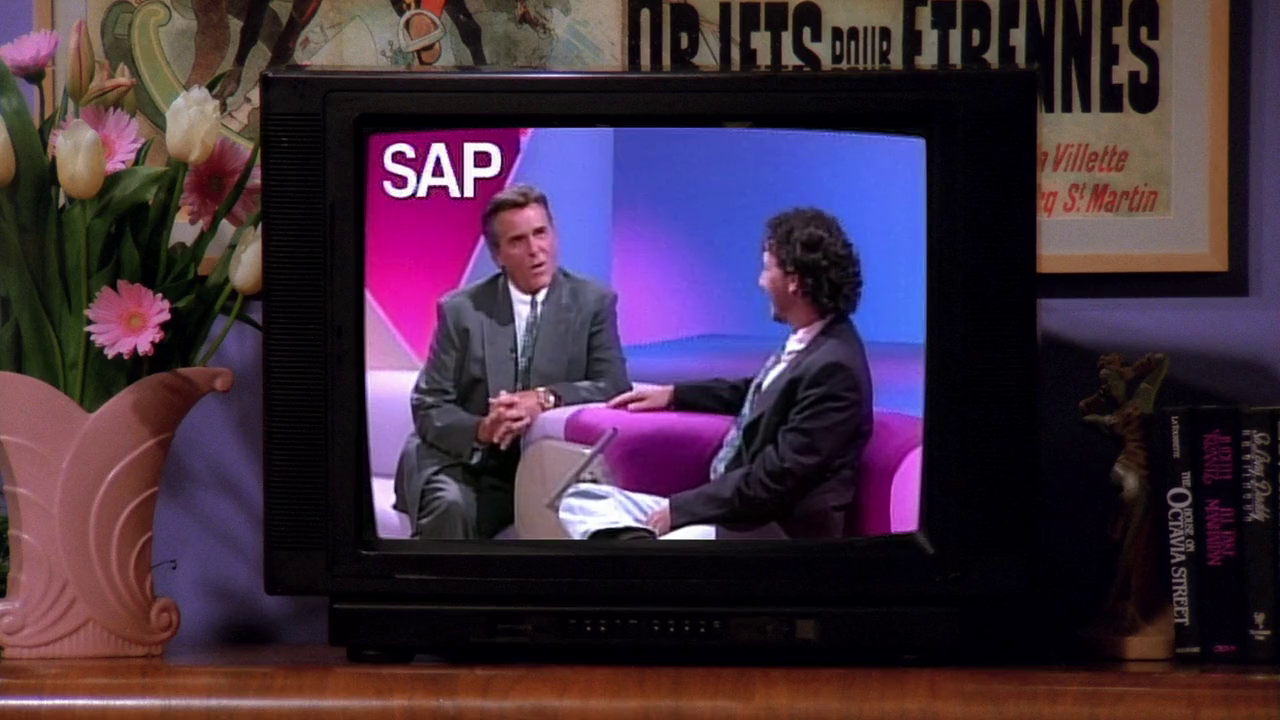
\includegraphics[trim={0 6cm 0 2cm,}, clip, width=\paperwidth]{./S01/img/17/love-connection.png}
    % \caption{Love Connection\label{fig:love-connection}}
  \end{adjustwidth}
\end{figure}

À espera dos doutores para um encontro, Rachel e Monica assistem a um
programa chamado \emph{Love Connection} (1983-1994), um programa de
encontros americano nos mesmos moldes de programas exibidos no SBT na
década de 90. Na época de lançamento do episódio, o \emph{Love
Connection} estava sendo reexibido. Na cena é possível ver o
apresentador \emph{Chuck Woolery} (1941-), à esquerda, conversando com
um participante.

\hypertarget{referuxeancias-2}{%
\subsection{Referências}\label{referuxeancias-2}}

\begin{itemize}
\tightlist
\item
  \sloppy Love Connection in Popular Culture - Fandom Wiki (Inglês). \url{https://gameshows.fandom.com/wiki/Love_Connection/In_Popular_Culture}
\item
  \sloppy Love Connection - Fandom Wiki (Inglês). \url{https://gameshows.fandom.com/wiki/Love_Connection}
\end{itemize}

\hypertarget{water-water-every-hare}{%
\section{Water, Water Every Hare}\label{water-water-every-hare}}

\begin{figure}[!ht]
  \begin{adjustwidth}{-\oddsidemargin-1in}{-\rightmargin}
    \centering
    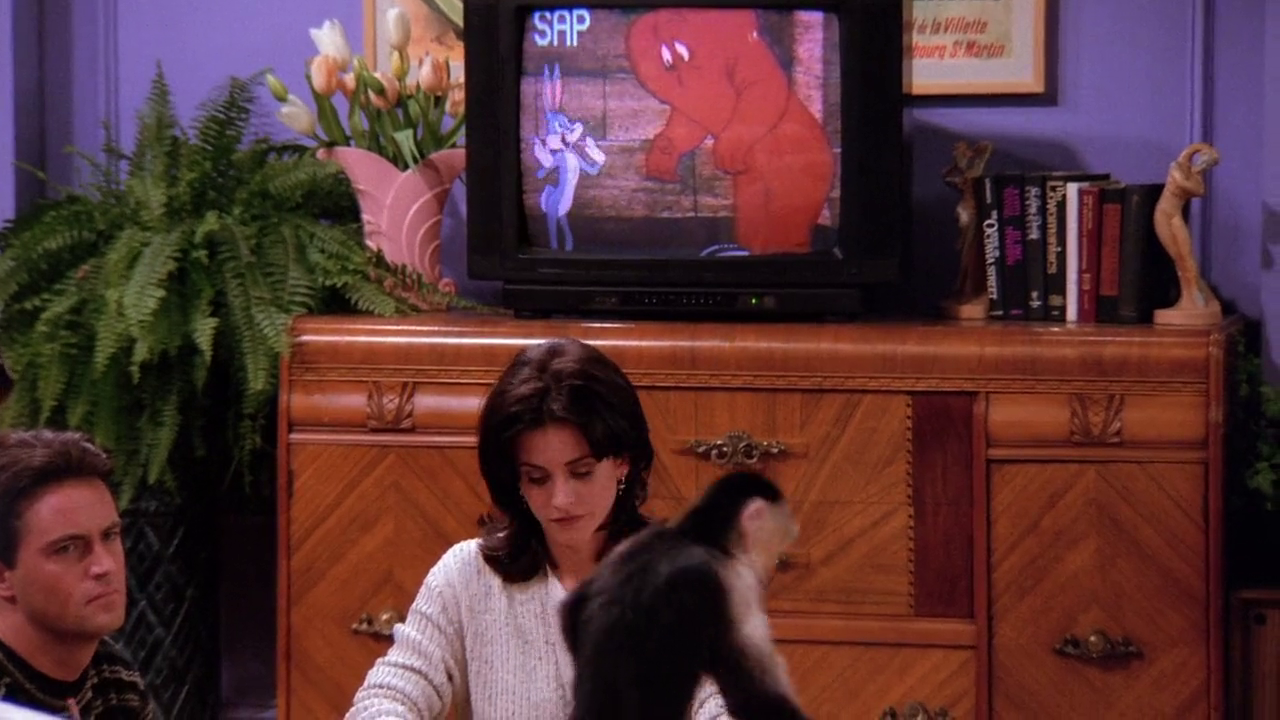
\includegraphics[trim={0 6cm 0 0cm,}, clip, width=\paperwidth]{./S01/img/17/water-water-every-hare.png}
    % \caption{Water, Water Every Hare\label{fig:water-water-every-hare}}
  \end{adjustwidth}
\end{figure}

Os amigos assistem ao episódio \emph{Water, Water Every Hare} (1952) do
\emph{Pernalonga}. O desenho ja foi citado no episódio
\textbf{\textcolor{primarycolor}{S01E03 - Aquele com o Dedão}}.

\hypertarget{referuxeancias-3}{%
\subsection{Referências}\label{referuxeancias-3}}

\begin{itemize}
\tightlist
\item
  \sloppy Water, Water Every Hare - Fandom Wiki (Inglês). \url{https://looneytunes.fandom.com/wiki/Water,_Water_Every_Hare}
\item
  \sloppy Vídeo - Dailymotion. \url{https://www.dailymotion.com/video/x2fgf28}
\end{itemize}

\hypertarget{scrabble}{%
\section{Scrabble}\label{scrabble}}

\begin{figure}[!ht]
  \begin{adjustwidth}{-\oddsidemargin-1in}{-\rightmargin}
    \centering
    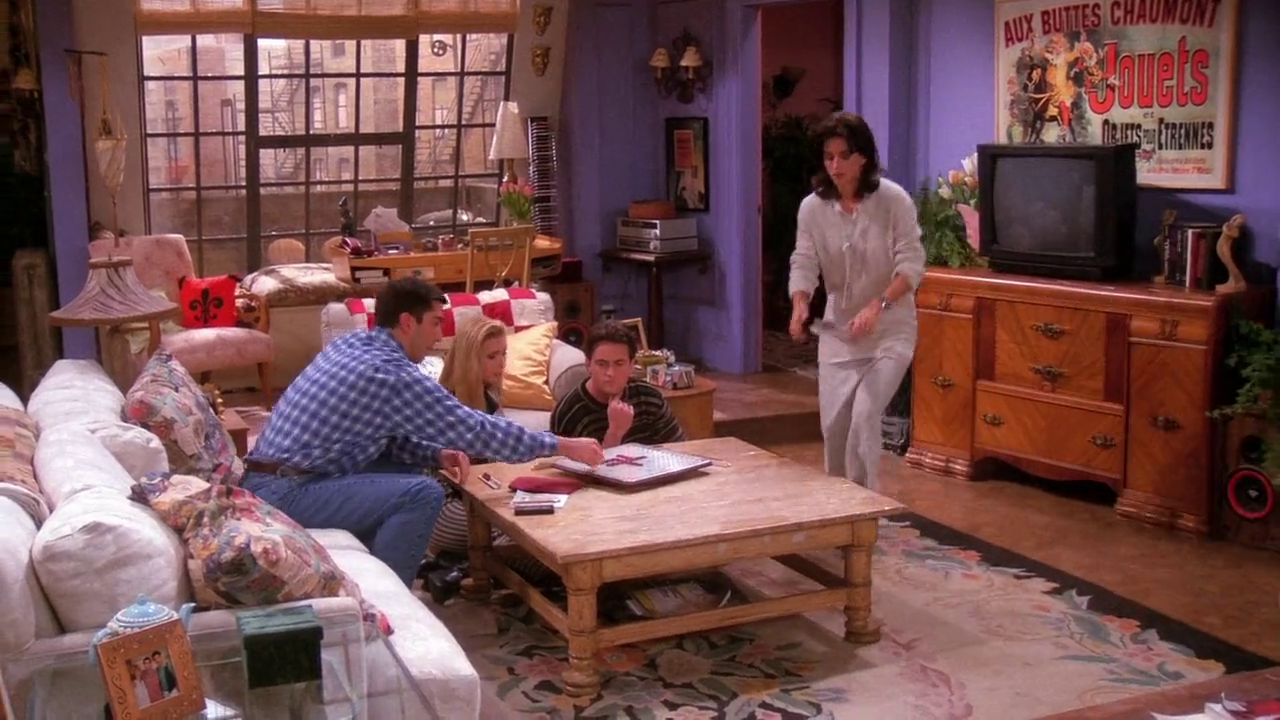
\includegraphics[trim={0 7cm 0 3cm,}, clip, width=\paperwidth]{./S01/img/17/scrabble.png}
    % \caption{Scrabble\label{fig:scrabble}}
  \end{adjustwidth}
\end{figure}

Nessa cena é possível ver os amigos jogando \emph{Scrabble} (1948), jogo
ao estilo palavras cruzadas em que os jogadores deve formar palavras
interligadas. É desse jogo que Marcel engole algumas peças e é levado ao
hospital.

\begin{figure}
  \centering
  \begin{tikzpicture}
    \node [inner sep=0pt] at (0,0) {
      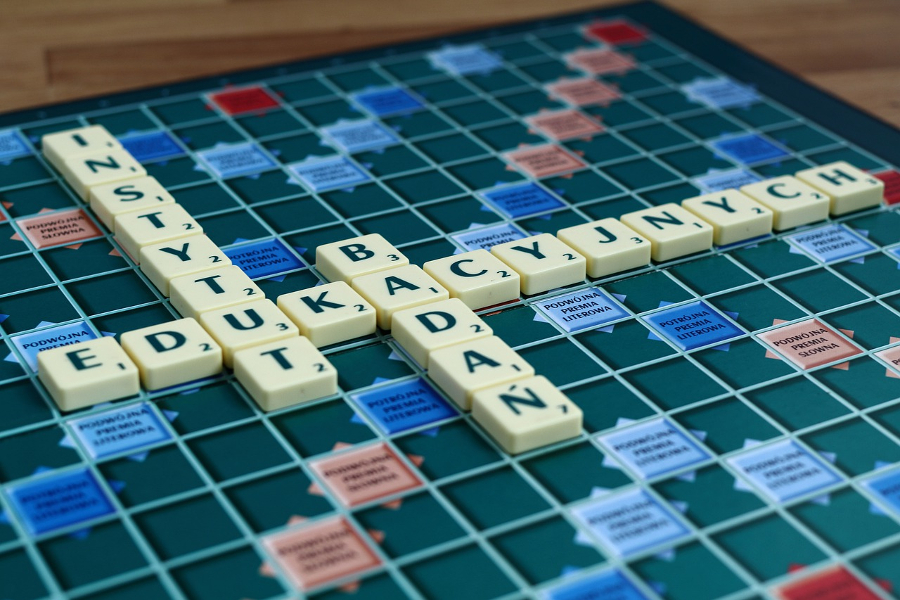
\includegraphics[width=0.8\textwidth,keepaspectratio]{./S01/img/17/scrabble-board.jpg}
    };
    \draw [white, rounded corners=\ClipSep, line width=\ClipSep]
    (current bounding box.north west) --
    (current bounding box.north east) --
    (current bounding box.south east) --
    (current bounding box.south west) -- cycle
    ;
    \end{tikzpicture}
    \caption{Scrabble - Tabuleiro\label{fig:scrabble-tabuleiro}}
\end{figure}

\hypertarget{referuxeancias-4}{%
\subsection{Referências}\label{referuxeancias-4}}

\begin{itemize}
\tightlist
\item
  \sloppy Scrabble - Encyclopædia Britannica. \url{https://www.britannica.com/sports/Scrabble}
\end{itemize}

\hypertarget{jeopardy}{%
\section{Jeopardy!}\label{jeopardy}}

\begin{figure}[!ht]
  \begin{adjustwidth}{-\oddsidemargin-1in}{-\rightmargin}
    \centering
    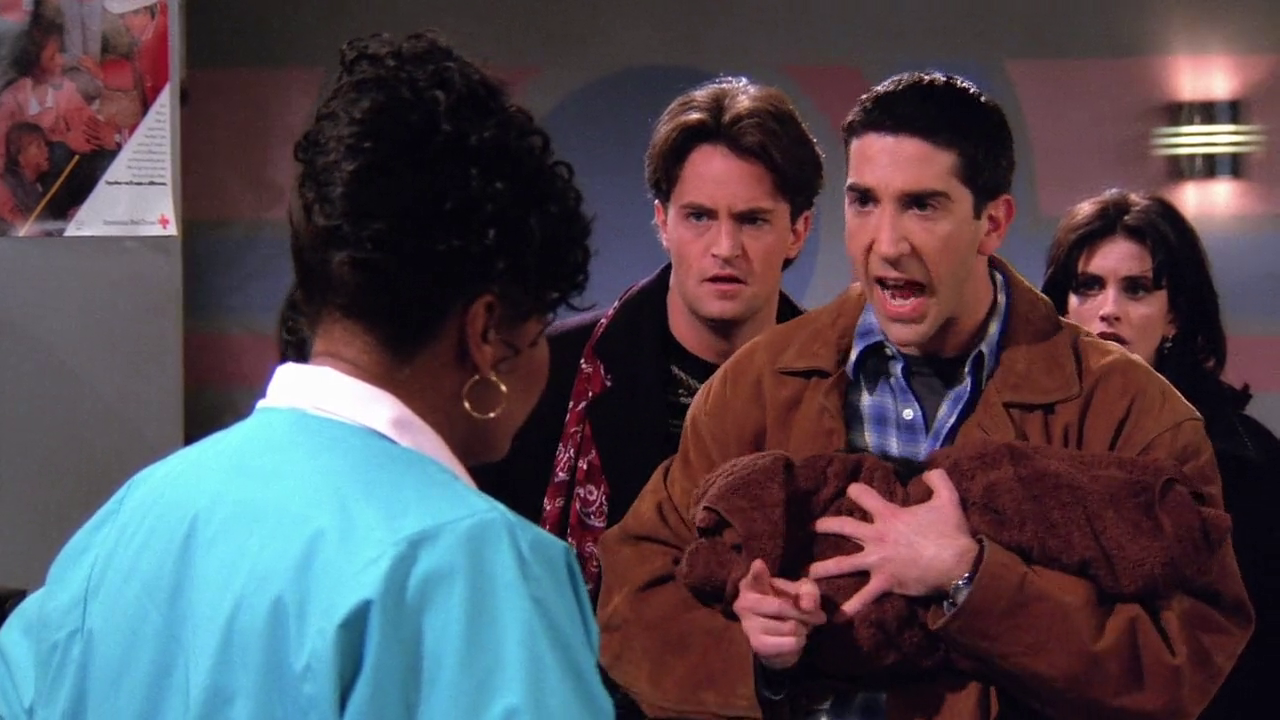
\includegraphics[trim={0 6cm 0 2cm,}, clip, width=\paperwidth]{./S01/img/17/jeopardy.png}
    % \caption{Jeopardy!\label{fig:jeopardy}}
  \end{adjustwidth}
\end{figure}

\begin{tcolorbox}[enhanced,center upper,
    drop fuzzy shadow southeast, boxrule=0.3pt,
    lower separated=false,
    colframe=black!30!dialogoBorder,colback=white]
\begin{minipage}[c]{0.16\linewidth}
  \raisebox{\dimexpr-\height+\ht\strutbox\relax}{
    \centering 
\includegraphics[width=1.4cm]{./assets/img/ross.png}
  }
   & \centering \scriptsize{Ross}
\end{minipage}
\hfill
\begin{minipage}[c]{0.8\linewidth}
  \textbf{- Lady, he is people. He has a name, okay? He watches Jeopardy...}\\
  - Senhora, ele é uma pessoa. Ele tem um nome, tá? Ele assiste Jeopardy...
\end{minipage}
\end{tcolorbox}

Com a esperança de que a recepcionista aceite que Marcel seja atendido
no hospital, Ross menciona que o símio assiste ao programa
\emph{Jeopardy!} (1964-), um programa de perguntas e respostas sobre
temas variados, onde são apresentadas as respostas e os competidores
devem formular as perguntas correspondentes.

\hypertarget{referuxeancias-5}{%
\subsection{Referências}\label{referuxeancias-5}}

\begin{itemize}
\tightlist
\item
  \sloppy Site oficial. \url{https://www.jeopardy.com/}
\item
  \sloppy Jeopardy! - Fandom Wiki. \url{https://gameshows.fandom.com/wiki/Jeopardy!}
\end{itemize}
